\documentclass[10pt]{beamer}
\usetheme[
%%% option passed to the outer theme
%    progressstyle=fixedCircCnt,   % fixedCircCnt, movingCircCnt (moving is deault)
  ]{Feather}
  
% If you want to change the colors of the various elements in the theme, edit and uncomment the following lines

% Change the bar colors:
\setbeamercolor{Feather}{bg=green!40!black}

% Change the color of the structural elements:
\setbeamercolor{structure}{fg=green!50!black}

% Change the frame title text color:
\setbeamercolor{frametitle}{fg=white}

% Change the normal text color background:
\setbeamercolor{normal text}{fg=green!30!black,bg=gray!80}

% Change the block colors
%\setbeamercolor{block title}{use=structure,fg=structure.fg,bg=structure.fg!20!bg}
\setbeamercolor{block title}{use=structure,fg=white,bg=structure.fg!20!bg}
%\setbeamercolor{block body}{parent=normal text,use=block title,bg=block title.bg!50!bg}
\setbeamercolor{block body}{parent=normal text,use=block title,bg=white}

%-------------------------------------------------------
% INCLUDE PACKAGES
%-------------------------------------------------------

\usepackage[utf8]{inputenc}
\usepackage[english]{babel}
\usepackage[T1]{fontenc}
\usepackage{helvet}
\usepackage{tabularx}
\usepackage{colortbl}

%-------------------------------------------------------
% DEFFINING AND REDEFINING COMMANDS
%-------------------------------------------------------

% colored hyperlinks
\newcommand{\chref}[2]{
  \href{#1}{{\usebeamercolor[bg]{Feather}#2}}
}

%-------------------------------------------------------
% INFORMATION IN THE TITLE PAGE
%-------------------------------------------------------

\title[Programming Merit Badge]{ }
\author{Joshua Talbot P.E.}
\institute{}
\date{28 November 2021}

%-------------------------------------------------------
% THE BODY OF THE PRESENTATION
%-------------------------------------------------------

\begin{document}

%-------------------------------------------------------
% THE TITLEPAGE
%-------------------------------------------------------

\section{Introduction}

{\1% % this is the name of the PDF file for the background

\begin{frame}{Programming Merit Badge}{ }
\begin{center}
\begin{block}{}
\center \textbf{Welcome!}
\end{block}
\vspace{0.5cm}
\begin{figure}%%Inicia paquete para cargar figura
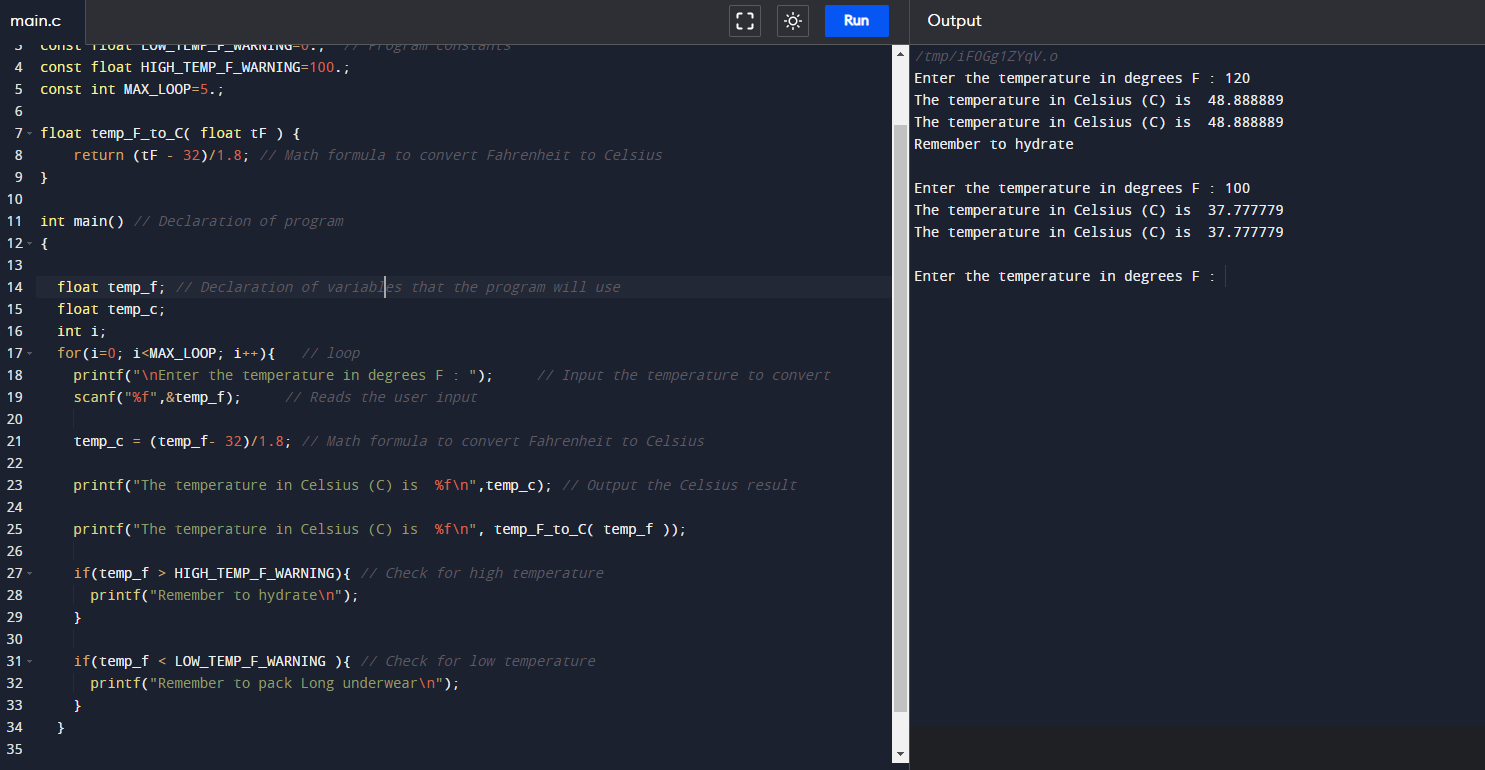
\includegraphics[width=\textwidth]{img/C_code.png}
%\caption{\label{fig:1}Programming}
\end{figure}
\end{center}
\end{frame}

%-------------------------------------------------------
% Cyber Chip
%-------------------------------------------------------

\begin{frame}{First Things First: Cyber Chip}{ }  
\begin{center}
\end{center}
\vskip 0.5cm

\begin{tabular}{m{0.4\linewidth}m{0.5\linewidth}}  

\includegraphics[width=0.3\textwidth]{img/cyberchip.png} & \cellcolor[gray]{0.8} Having a valid Cyber Chip is a prerequist for this merit badge.  Do you have one?  If not please get one before proceeding with this merit badge.
To get the Cyber Chip visit this link with your parents: {\footnotesize \url{https://www.scouting.org/training/youth-protection/cyber-chip/}}
\end{tabular} 
\vspace{1cm}

\end{frame}

%-------------------------------------------------------
% Required Resources
%-------------------------------------------------------

\begin{frame}{Required Tools and Resources}{}
\begin{block}{}
  \begin{itemize}
    \item {\tt Valid Cyber Chip to perform research and web based programming}
    \item {\tt Programming Merit Badge Workbook \url{http://usscouts.org/mb/worksheets/programming.pdf}}
    \item {\tt Computer (Chromebook, Laptop, Desktop) with internet connection\footnote{Talk to me if you don't have a computer that can be used.}}
    \vspace{2cm}
    \end{itemize}
	\end{block}
\end{frame}

%-------------------------------------------------------
% Safety Resources
%-------------------------------------------------------

\begin{frame}{Safety Resources}{}
\begin{block}{}
  \begin{itemize}
    \item {\tt Computer-related injuries \url{https://www.betterhealth.vic.gov.au/health/healthyliving/computer-related-injuries}}
    \item {\tt Ergonomics \& Computer Use \url{https://uhs.princeton.edu/health-resources/ergonomics-computer-use}}
    \end{itemize}
  \end{block}
\end{frame}

%-------------------------------------------------------
% History Resources
%-------------------------------------------------------

\begin{frame}{Programming Historical Resources}{}
  \begin{block}{}
    \begin{itemize}
      \item {\tt History of programming languages \url{https://en.wikipedia.org/wiki/History_of_programming_languages}}
      \item {\tt Evolution of programming languages\url{https://en.wikipedia.org/wiki/Programming_language_generations}}
      \item {\tt Ask a parent for their option on the history or programming or computers.}
    \end{itemize}
  \end{block}
\end{frame}

%-------------------------------------------------------
% General Knowledge Resources
%-------------------------------------------------------

\begin{frame}{General Knowledge Resources}{}
\begin{block}{}
  \begin{itemize}
    \item {\tt Valid Cyber Chip to perform research and web based programming}
    \item {\tt Popular Languages \url{https://www.northeastern.edu/graduate/blog/most-popular-programming-languages/}}
    \item {\tt Evolution of Languages \url{https://www.geeksforgeeks.org/the-evolution-of-programming-languages/}}
    \item {\tt TIOBE Index \url{https://www.tiobe.com/tiobe-index/}}
    \end{itemize}
  \end{block}
\end{frame}

%-------------------------------------------------------
% Intellectual Property Resources
%-------------------------------------------------------

\begin{frame}{Intellectual Property (I.P.) Resources}{}
\begin{block}{Merit Badge Requirements for I.P.}
The merit badge is looking for 4 methods to protect intellectual property (IP).

One of these methods will not protect a "program".  However this method is used to protect certain forms of I.P. and therefore is included on this topic of the merit badge.

Can you figure out which of the 4 can't be used to protect the I.P. of a software program?
\end{block}
\begin{block}{I.P. Resources}
  \begin{itemize}
    \item {\tt 4 forms of Software Intellectual Property \url{https://cpl.thalesgroup.com/software-monetization/protecting-software-intellectual-property}}
    \end{itemize}
  \end{block}
\end{frame}

%-------------------------------------------------------
% Software License Resources
%-------------------------------------------------------

\begin{frame}{Software License Resources}{}
\begin{block}{License Resources}
  \begin{itemize}
    \item {\tt Software Licenses \url{https://en.wikipedia.org/wiki/Software_license}}
    \item {\tt Open Source License \url{https://en.wikipedia.org/wiki/Open-source_software}}
    \item {\tt Freeware License \url{https://en.wikipedia.org/wiki/Freeware}}
    \item {\tt Proprietary software \url{https://en.wikipedia.org/wiki/Proprietary_software}\footnote{I belive the BSA intended to use the term `proprietary', not `commercial'. Today some commercial software is open or free or is converted from proprietary to open source.}}
  \end{itemize}
\end{block}
\end{frame}

%-------------------------------------------------------
% Programming Resources
%-------------------------------------------------------

\begin{frame}{Resources related to Programming}{}
\begin{block}{Resources}
  \begin{itemize}
    \item {\tt Scout Life: Programming merit badge \url{https://scoutlife.org/merit-badges/programming-merit-badge/}}
    \item {\tt BSA - VEX Robotic Arm Video \url{https://www.youtube.com/watch?v=BbKn5G7-gGY}}
    \item {\tt BSA - Arduino Example Video\footnote{\label{ard_rqd}This requires an Arduino.} \url{https://www.youtube.com/watch?v=YZrclRnf3Ho}}
    
    \end{itemize}
  \end{block}
\end{frame}

%-------------------------------------------------------
% Start Programming
%-------------------------------------------------------

\begin{frame}{Actual Programming}{}
\begin{block}{Resources Part 1}
  \begin{itemize}
    \item {\tt Programiz - resources and examples for the popular \url{https://www.programiz.com/}}
    \item {\tt Coding Ground - several offerings \url{https://www.tutorialspoint.com/codingground.htm}}
    \item {\tt Arduino for Beginners Video\footnote{\label{ard_rqd}This requires an Arduino.} \url{https://www.youtube.com/watch?v=fJWR7dBuc18}}
    \item {\tt Learn Pyhton \url{https://www.learnpython.org/}}
    \item {\tt Learn HTML \url{https://www.codecademy.com/learn/learn-html}}
    \item {\tt Scratch \url{https://scratch.mit.edu/} or \url{https://inventwithscratch.com/}}
    \end{itemize}
  \end{block}
\end{frame}

%-------------------------------------------------------
% Start Programming
%-------------------------------------------------------

\begin{frame}{Actual Programming}{}
\begin{block}{Resources Part 2}
  \begin{itemize}
    \item {\tt PyGame (Games written using Python) \url{https://www.pygame.org/news} or \url{http://inventwithpython.com/pygame/}}
    \item {\tt Learn JavaScript \url{https://www.codecademy.com/learn/introduction-to-javascript}}
    \item {\tt Build a Mobile App (Scratch like environment) \url{https://appinventor.mit.edu/}}
    \item  {\tt CoderDojo \url{https://projects.raspberrypi.org/en/coderdojo}}
    \item {\tt Tons of Projects using a RaspberryPi and other inexpensive hardware \url{https://projects.raspberrypi.org/en/projects}}
    \item {\tt Quick Summary of almost all... \url{https://learnxinyminutes.com/}}
    \end{itemize}
  \end{block}
\end{frame}

%-------------------------------------------------------
% Programming Tips
%-------------------------------------------------------

\begin{frame}{Tips to Programming}{}
\begin{block}{}
  \begin{itemize}
    \item {Start Small}
    \item {Veteran programmers generally don't start from scratch.  They build on something already started.  I would encourage you to do the same.}
    \item {Test often - VERY often!!!}
    \item {Don't give in.  Errors can be very hard to decipher.  If you can't figure it out, comment stuff out until it works again to narrow down the issue.  This is why we test OFTEN!}
    \end{itemize}
  \end{block}
\end{frame}

%-------------------------------------------------------
% Completing the Requirements
%-------------------------------------------------------

\begin{frame}{Tips to completing the requirements}{}
\begin{block}{Part 1}
This merit badge requires you to use 3 languages, the first task is to modify a existing program.  The second and third tasks require you to create your own program.  Modifing an existing program is one of the best ways to learn how to create a program and would encourage you to modify several different programs from 3 or more languages.  Develop a program of your own from two of programming languages you like the best of the ones you tried.  Use the third language to complete the first requirement.
  \begin{itemize}
    \item {Try several different languages to see which ones you like the best.}
    \item {Scratch, HTML, Python are the `easier' languages.}
    \item {C, C++, Java are `harder' because they are more syntax strict.}
    \end{itemize}

  %My favorite languages are C and Python.  Bot of these are very powerful for very different reasons.  C is fast and can be compiled to run on almost every computer or device ever created.  Python has a VERY large following and has a immense library of tools to do almost anything you can think of fairly easily, however Python is an interpreted language so it requires a large amount of resources and is not suitable to run on small embedded devices like the Arduino (at least not yet). 
  \end{block}
\end{frame}

%-------------------------------------------------------
% Completing the Requirements
%-------------------------------------------------------

\begin{frame}{Tips to completing the requirements}{}
\begin{block}{Part 2}
  \begin{itemize}
    \item {\tt One of the best ways to learn a new programming language is to find an example and modify it to see how the language works.  Try it on Scratch, Python and HTML to see which of these two you want to use for requirements 5b and 5c.}
    \item {\tt Remember build on something already started.  Professioanl prgrammers do the same.  They hardly ever start from stratch.}
    \item {\tt Plan out the project first, not after. }
    \item {\tt Start small then build new features into an already working project.  Shooting for the moon on day 1 will result in failure.  Learn to lift one leg first. }
    \end{itemize}
  \end{block}
\end{frame}

%-------------------------------------------------------
% Programming Ideas
%-------------------------------------------------------

\begin{frame}{Some Programming Ideas}{}
\begin{block}{}
  \begin{itemize}
    \item Traffic light controller (red, green and yellow lights, switch states when car is present).
    \item Rock, Paper, Scissors Game.
    \item Odd or Even Game.
    \item Entry detection system: monitor input and sound an alarm if broken.
    \item Family web page - Family page + your personal page.
    \item Unit conversion (gallons to cups, feet to miles)
    \item Hiking Time estimator (input distance, pace and elevation to determine total trek time).
    \item 
    \end{itemize}
  \end{block}
\end{frame}

%-------------------------------------------------------
% Contact Information
%-------------------------------------------------------

\begin{frame}{Contact}{}
\begin{block}{}
Below is my contact information.  I prefer email over a phone call, however in an emergency please call.  When emailing always be sure to `CC' your parent or one of the other adult leaders on all emails.  If you call my phone, please have your parent present with you.
\end{block}
\begin{block}{}
Name: Josh Talbot

Email: talbot.j@gmail.com

Phone: 585-794-1708
\end{block}
\begin{block}{}
I know the following languages - do not let this deter you from learning others, but I can provide help with the following: Arduino (C/C++), C, C++, Javascript, Labview, Ladder Logic, Matlab (Octave), PHP, Python, Scratch, Simulink, SQL, Visual Basic, VBA, VB.Net.  Many languages are very similar and should be able to help/guide almost any other common language.
\end{block}
\end{frame}

{\1
\begin{frame}
  \begin{block}{}
  {\huge Good Luck with the Programming!}
  \end{block}
\end{frame}}
\end{document}